\appendix
\chapter{MT50 Action-Bounding Per-Task Details}
\label{app:action-audit-per-task}

Table~\ref{tab:action-audit-per-task} lists per-task MT50 action-bounding audit metrics for all 50 MetaWorld tasks (25 episodes each, seeds 1000--1024). Column meanings are: \textbf{Task}, MetaWorld task name (without the \texttt{-v3} suffix); \textbf{Diff.}, manual difficulty bucket; \textbf{Winner}, branch with more latent-comparison column wins; \textbf{Success}, successful real-environment episodes out of 25; \textbf{Raw}, \textbf{Bounded}, and \textbf{Ties}, percentages of comparison columns where raw actions, bounded actions, or neither branch had lower latent L2; \textbf{Raw L2} and \textbf{Bounded L2}, mean combined visual-plus-proprio latent L2 for each branch; \textbf{$\Delta$ B-R}, bounded mean L2 minus raw mean L2 (negative favours bounded); \textbf{Avg steps}, mean episode length; \textbf{Avg seg.}, mean number of 50-action chunks per episode; \textbf{Avg reward} and \textbf{Max reward}, mean episode return and mean maximum per-step reward; \textbf{Cols}, number of latent comparison columns; \textbf{Min}, minimum observed combined L2.

\begin{landscape}
\small
\begin{longtable}{@{}l l l r r r r r r r r r r r r r@{}}
\caption{Per-task MT50 action-bounding audit details.}\label{tab:action-audit-per-task}\\
\toprule
Task & Diff. & Winner & Success & Raw & Bounded & Ties & Raw L2 & Bounded L2 & $\Delta$ B-R & Avg steps & Avg seg. & Avg reward & Max reward & Cols & Min \\ 
\midrule
\endfirsthead
\toprule
Task & Diff. & Winner & Success & Raw & Bounded & Ties & Raw L2 & Bounded L2 & $\Delta$ B-R & Avg steps & Avg seg. & Avg reward & Max reward & Cols & Min \\ 
\midrule
\endhead
assembly & hard & bounded & 1/25 & 40.89\% & 56.82\% & 2.29\% & 279.8 & 274.9 & -4.9 & 148.2 & 3.0 & 157.2 & 3.1 & 741 & 6.3 \\
basketball & medium & bounded & 5/25 & 26.28\% & 73.72\% & 0.00\% & 332.5 & 292.9 & -39.6 & 140.2 & 2.9 & 90.5 & 2.5 & 704 & 5.8 \\
bin-picking & medium & bounded & 7/25 & 20.99\% & 76.82\% & 2.19\% & 267.7 & 240.1 & -27.6 & 136.6 & 2.8 & 28.9 & 2.9 & 686 & 5.8 \\
box-close & medium & bounded & 1/25 & 43.62\% & 55.17\% & 1.21\% & 301.9 & 290.1 & -11.8 & 148.9 & 3.0 & 96.0 & 2.8 & 745 & 6.3 \\
button-press-topdown & easy & bounded & 22/25 & 6.60\% & 93.40\% & 0.00\% & 594.6 & 228.6 & -365.9 & 77.3 & 2.1 & 171.2 & 5.2 & 394 & 4.0 \\
button-press-topdown-wall & easy & bounded & 24/25 & 5.08\% & 94.92\% & 0.00\% & 688.4 & 240.6 & -447.9 & 61.0 & 2.0 & 0.4 & 0.0 & 315 & 3.6 \\
button-press & easy & bounded & 24/25 & 1.86\% & 98.14\% & 0.00\% & 470.7 & 221.6 & -249.1 & 62.4 & 2.0 & 44.3 & 1.5 & 323 & 3.5 \\
button-press-wall & easy & bounded & 20/25 & 17.48\% & 81.82\% & 0.70\% & 289.1 & 238.4 & -50.7 & 84.5 & 2.2 & 168.9 & 6.3 & 429 & 4.2 \\
coffee-button & easy & bounded & 21/25 & 12.64\% & 86.99\% & 0.37\% & 322.1 & 263.6 & -58.5 & 51.9 & 1.3 & 32.8 & 1.1 & 269 & 3.3 \\
coffee-pull & medium & bounded & 11/25 & 37.10\% & 53.98\% & 8.92\% & 306.0 & 270.4 & -35.6 & 124.9 & 2.6 & 23.0 & 1.1 & 628 & 5.7 \\
coffee-push & medium & bounded & 7/25 & 37.02\% & 48.24\% & 14.74\% & 271.5 & 269.2 & -2.3 & 124.4 & 2.7 & 16.5 & 1.0 & 624 & 5.5 \\
dial-turn & easy & bounded & 7/25 & 38.90\% & 61.10\% & 0.00\% & 287.9 & 284.9 & -3.0 & 126.5 & 2.7 & 225.9 & 5.3 & 635 & 5.5 \\
disassemble & very\_hard & bounded & 3/25 & 39.89\% & 55.65\% & 4.46\% & 296.6 & 277.3 & -19.3 & 143.2 & 2.9 & 76.6 & 2.2 & 717 & 6.1 \\
door-close & easy & bounded & 25/25 & 0.32\% & 99.68\% & 0.00\% & 756.8 & 289.8 & -466.9 & 61.7 & 2.0 & 94.1 & 8.6 & 316 & 3.2 \\
door-lock & easy & bounded & 6/25 & 15.73\% & 84.27\% & 0.00\% & 483.2 & 348.0 & -135.2 & 130.6 & 2.8 & 233.4 & 3.8 & 655 & 5.7 \\
door-open & easy & bounded & 17/25 & 24.08\% & 75.73\% & 0.19\% & 486.2 & 291.8 & -194.4 & 101.7 & 2.3 & 307.4 & 8.1 & 515 & 4.7 \\
door-unlock & easy & raw & 15/25 & 57.85\% & 42.15\% & 0.00\% & 312.8 & 320.2 & +7.4 & 84.0 & 1.8 & 153.4 & 6.2 & 427 & 4.2 \\
drawer-close & easy & bounded & 25/25 & 17.04\% & 82.96\% & 0.00\% & 604.6 & 318.8 & -285.8 & 78.8 & 2.0 & 26.1 & 10.0 & 405 & 3.7 \\
drawer-open & easy & raw & 16/25 & 66.21\% & 33.45\% & 0.34\% & 237.4 & 247.9 & +10.5 & 114.5 & 2.4 & 294.0 & 6.5 & 580 & 5.1 \\
faucet-close & easy & bounded & 22/25 & 5.26\% & 94.74\% & 0.00\% & 553.3 & 245.7 & -307.7 & 70.7 & 2.1 & 271.3 & 9.3 & 361 & 3.9 \\
faucet-open & easy & bounded & 24/25 & 2.31\% & 97.69\% & 0.00\% & 526.4 & 280.4 & -246.0 & 58.8 & 2.0 & 235.0 & 9.8 & 303 & 3.5 \\
hammer & medium & raw & 0/25 & 51.33\% & 43.87\% & 4.80\% & 306.5 & 300.5 & -6.0 & 150.0 & 3.0 & 145.8 & 1.1 & 750 & 6.2 \\
hand-insert & hard & raw & 3/25 & 62.95\% & 30.33\% & 6.72\% & 269.7 & 276.2 & +6.5 & 139.7 & 2.9 & 30.3 & 1.9 & 699 & 5.8 \\
handle-press-side & easy & bounded & 23/25 & 0.40\% & 99.60\% & 0.00\% & 648.8 & 242.7 & -406.1 & 48.7 & 1.2 & 64.0 & 9.3 & 252 & 2.9 \\
handle-press & easy & bounded & 24/25 & 0.00\% & 100.00\% & 0.00\% & 709.7 & 230.9 & -478.8 & 30.0 & 1.1 & 28.5 & 9.6 & 160 & 2.5 \\
handle-pull-side & easy & bounded & 0/25 & 22.00\% & 77.87\% & 0.13\% & 420.8 & 235.9 & -184.9 & 150.0 & 3.0 & 23.3 & 0.7 & 750 & 6.0 \\
handle-pull & easy & bounded & 0/25 & 34.00\% & 66.00\% & 0.00\% & 387.4 & 303.7 & -83.6 & 150.0 & 3.0 & 33.0 & 2.7 & 750 & 6.1 \\
lever-pull & easy & bounded & 11/25 & 34.32\% & 65.68\% & 0.00\% & 318.4 & 287.7 & -30.7 & 120.7 & 2.6 & 153.9 & 3.9 & 609 & 5.6 \\
peg-insert-side & medium & bounded & 1/25 & 18.72\% & 79.51\% & 1.76\% & 379.3 & 266.2 & -113.2 & 147.4 & 3.0 & 12.9 & 0.7 & 737 & 5.9 \\
peg-unplug-side & easy & bounded & 5/25 & 32.12\% & 55.18\% & 12.70\% & 293.9 & 269.7 & -24.2 & 136.6 & 2.8 & 40.0 & 1.5 & 685 & 5.8 \\
pick-out-of-hole & hard & bounded & 6/25 & 27.03\% & 72.55\% & 0.43\% & 324.3 & 278.5 & -45.8 & 140.3 & 2.9 & 40.7 & 1.8 & 703 & 5.9 \\
pick-place & hard & bounded & 4/25 & 47.85\% & 49.04\% & 3.11\% & 249.0 & 250.1 & +1.1 & 134.8 & 2.8 & 60.8 & 1.5 & 675 & 5.4 \\
pick-place-wall & very\_hard & raw & 7/25 & 48.85\% & 48.70\% & 2.44\% & 364.5 & 275.5 & -89.0 & 130.2 & 2.7 & 78.6 & 2.3 & 655 & 5.5 \\
plate-slide-back-side & easy & raw & 16/25 & 54.72\% & 45.28\% & 0.00\% & 290.5 & 293.1 & +2.6 & 83.3 & 1.9 & 93.8 & 5.6 & 424 & 4.0 \\
plate-slide-back & easy & bounded & 0/25 & 42.00\% & 57.87\% & 0.13\% & 278.1 & 276.3 & -1.8 & 150.0 & 3.0 & 67.7 & 1.6 & 750 & 6.1 \\
plate-slide-side & easy & bounded & 22/25 & 0.94\% & 99.06\% & 0.00\% & 316.1 & 288.4 & -27.7 & 61.8 & 1.4 & 170.0 & 7.7 & 319 & 3.4 \\
plate-slide & easy & bounded & 19/25 & 31.05\% & 68.95\% & 0.00\% & 260.2 & 247.1 & -13.1 & 80.5 & 2.2 & 148.3 & 6.3 & 409 & 4.0 \\
push-back & hard & raw & 9/25 & 51.74\% & 45.89\% & 2.37\% & 292.4 & 296.5 & +4.1 & 125.7 & 2.7 & 11.9 & 1.0 & 632 & 5.4 \\
push & hard & raw & 5/25 & 48.19\% & 44.41\% & 7.40\% & 235.5 & 237.2 & +1.8 & 131.6 & 2.8 & 48.4 & 2.6 & 662 & 5.5 \\
push-wall & medium & bounded & 9/25 & 36.84\% & 61.72\% & 1.44\% & 419.3 & 266.7 & -152.6 & 124.9 & 2.6 & 93.5 & 3.4 & 627 & 5.1 \\
reach & easy & bounded & 10/25 & 22.62\% & 56.91\% & 20.47\% & 259.1 & 251.4 & -7.7 & 110.8 & 2.4 & 704.4 & 9.0 & 557 & 4.9 \\
reach-wall & easy & bounded & 7/25 & 33.60\% & 50.08\% & 16.32\% & 300.5 & 265.5 & -34.9 & 125.5 & 2.6 & 709.6 & 8.6 & 631 & 5.3 \\
shelf-place & very\_hard & bounded & 1/25 & 14.63\% & 85.23\% & 0.14\% & 426.4 & 258.5 & -167.8 & 147.6 & 3.0 & 13.5 & 0.6 & 738 & 6.0 \\
soccer & medium & bounded & 4/25 & 30.26\% & 69.74\% & 0.00\% & 248.8 & 244.0 & -4.8 & 136.4 & 2.8 & 74.5 & 2.0 & 684 & 5.7 \\
stick-pull & very\_hard & raw & 1/25 & 64.41\% & 35.18\% & 0.41\% & 325.2 & 339.0 & +13.8 & 147.6 & 3.0 & 37.8 & 1.1 & 739 & 5.8 \\
stick-push & very\_hard & raw & 8/25 & 49.84\% & 47.65\% & 2.51\% & 325.8 & 332.8 & +7.0 & 127.0 & 2.7 & 27.7 & 1.7 & 638 & 5.4 \\
sweep-into & medium & bounded & 11/25 & 31.95\% & 68.05\% & 0.00\% & 302.8 & 264.5 & -38.3 & 104.7 & 2.2 & 56.1 & 5.3 & 529 & 4.9 \\
sweep & medium & bounded & 8/25 & 16.80\% & 83.20\% & 0.00\% & 560.5 & 349.6 & -210.9 & 129.1 & 2.7 & 89.6 & 4.1 & 649 & 5.5 \\
window-close & easy & bounded & 25/25 & 28.40\% & 71.60\% & 0.00\% & 595.0 & 283.0 & -312.0 & 79.7 & 2.0 & 126.0 & 7.6 & 412 & 3.8 \\
window-open & easy & bounded & 24/25 & 37.69\% & 62.31\% & 0.00\% & 560.1 & 329.4 & -230.7 & 91.0 & 2.1 & 84.9 & 4.6 & 467 & 4.3 \\
\bottomrule
\end{longtable}
\normalsize
\end{landscape}

\chapter{Action-Bounding Decode Strips}

\IfFileExists{appendix/figures/phase57_drawer_open_ep0000_seg0001_strip_l2.png}{%
\begin{figure}[ht]
\centering
\includegraphics[width=\linewidth]{appendix/figures/phase57_drawer_open_ep0000_seg0001_strip_l2.png}
\caption{Action-bounding decode strip for \texttt{drawer-open-v3} (episode seed 1000, segment 1).
SmolVLA sampled a 50-step action chunk; the real environment was stepped with the raw postprocessed actions.
From the same root observation, the JEPA world model was unrolled with raw actions (middle row) and with clipped/bounded actions (bottom row).
The top row shows aligned real camera frames.
Per-column labels report combined visual-plus-proprio L2 distance to the real latent; lower L2 means the world model prediction is closer to what actually happened.}
\label{fig:appendix-action-audit-drawer-open-seg1}
\end{figure}
}{}

\IfFileExists{appendix/figures/phase57_drawer_close_ep0001_seg0001_strip_l2.png}{%
\begin{figure}[ht]
\centering
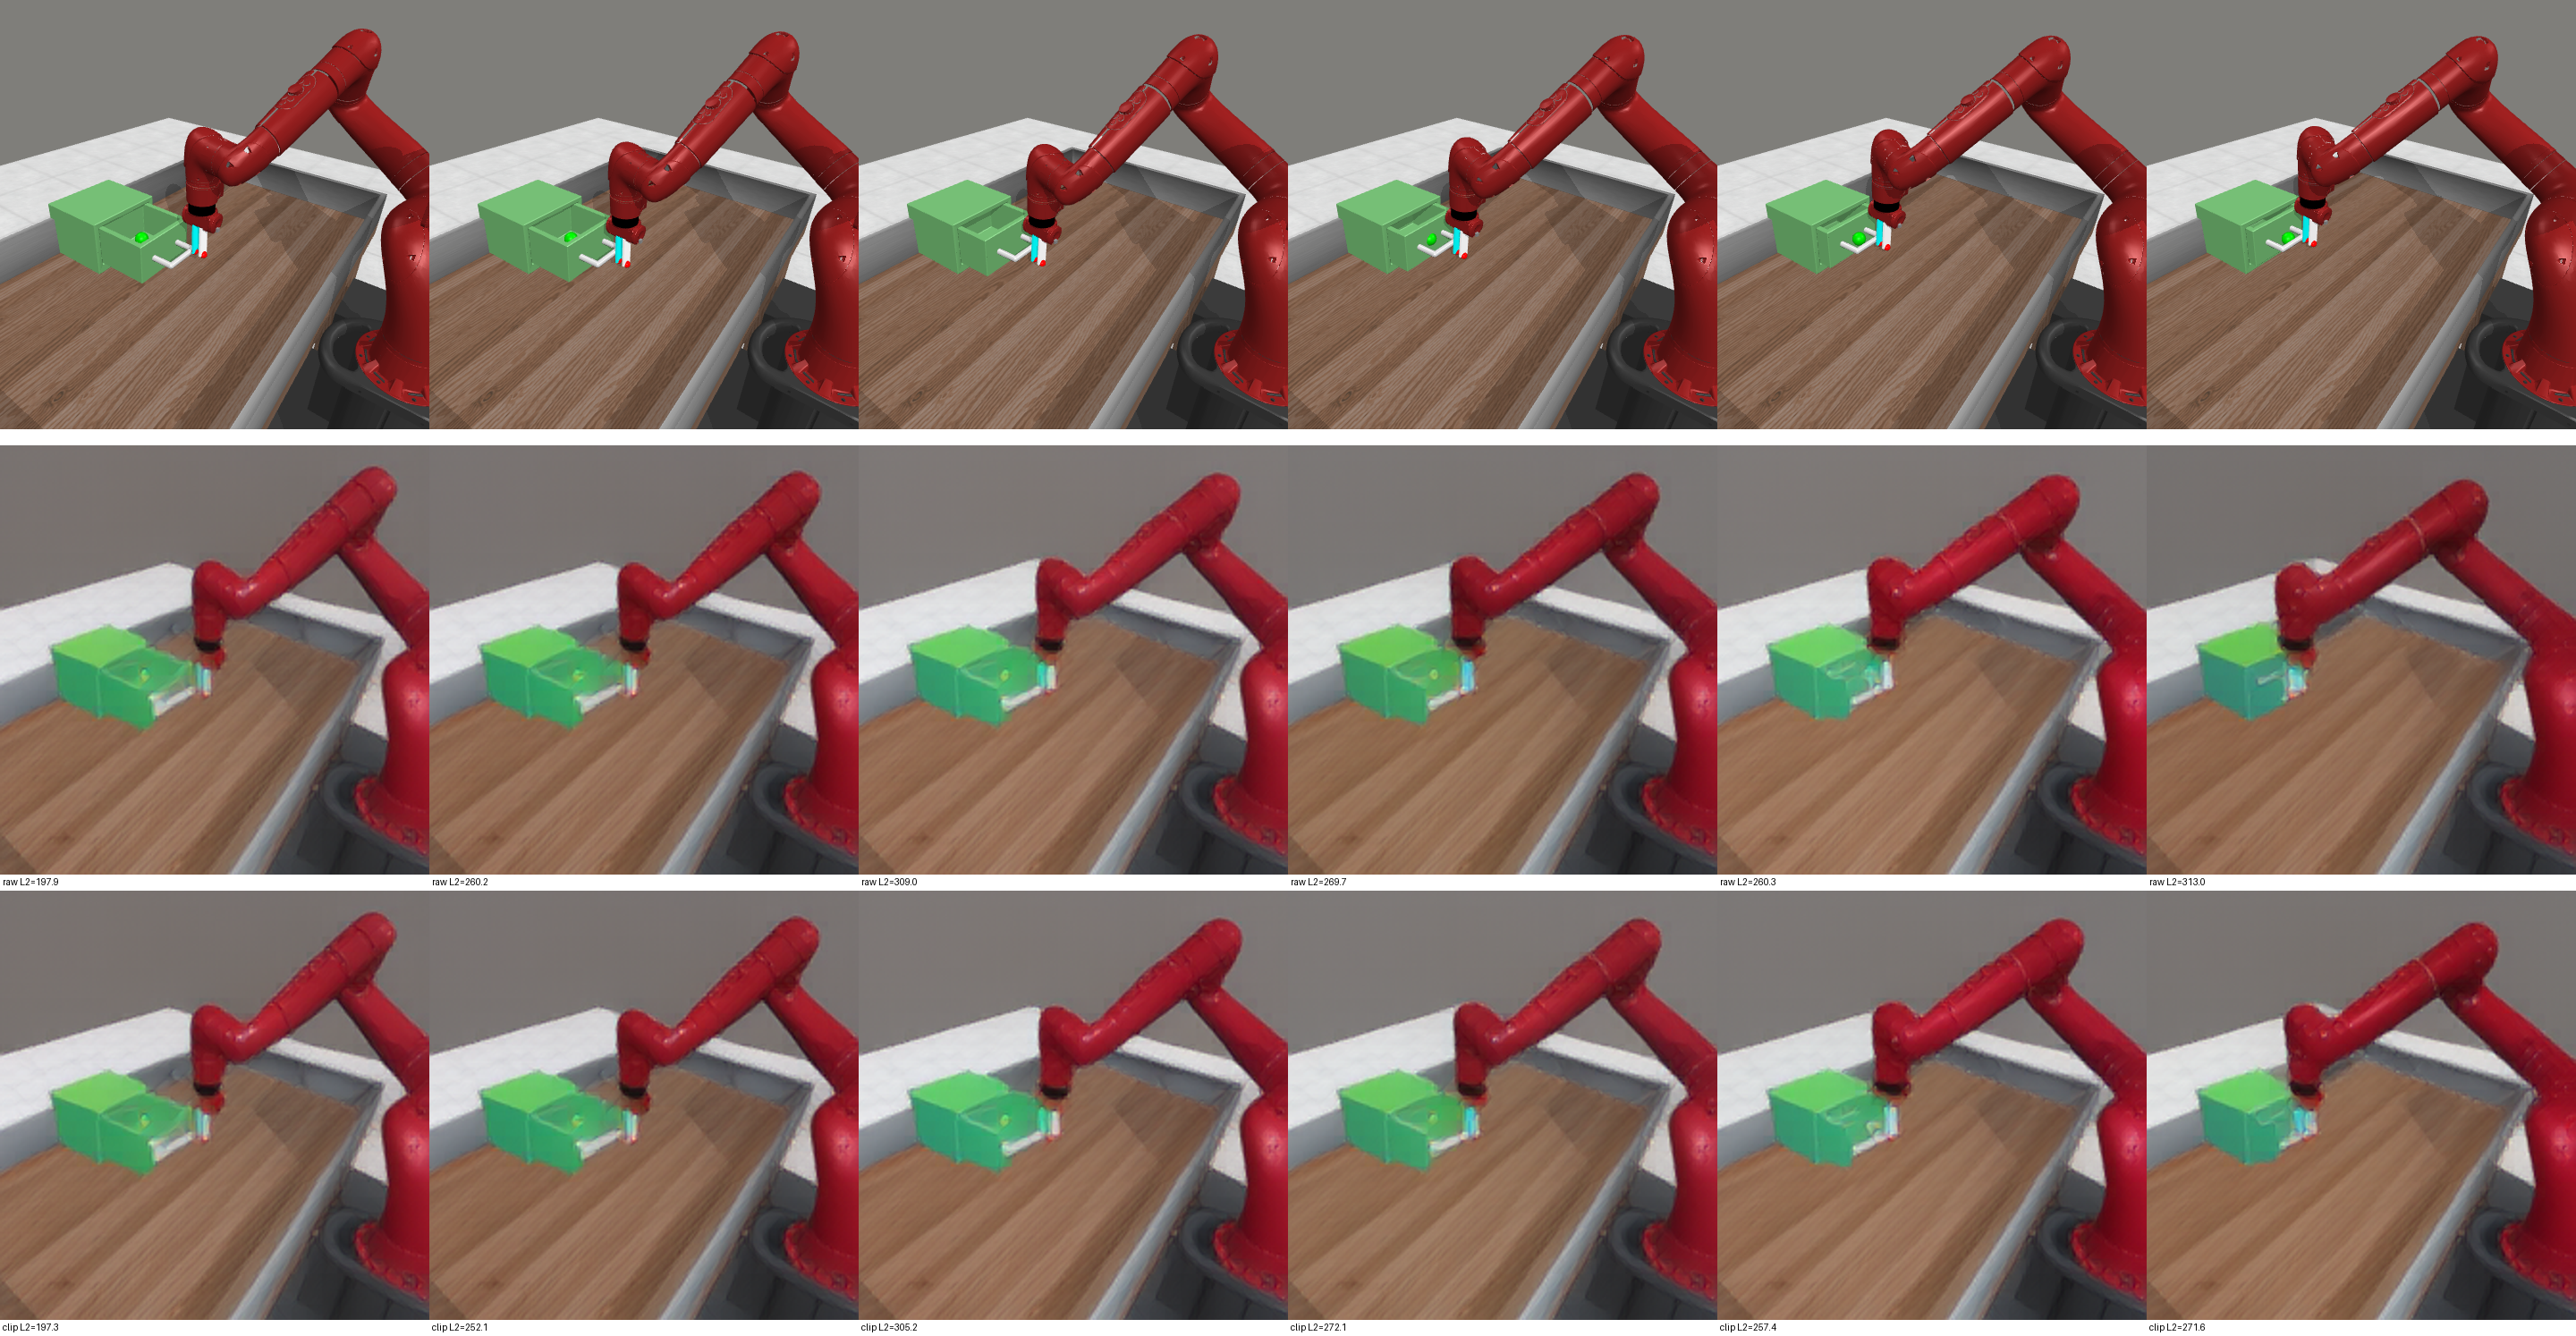
\includegraphics[width=\linewidth]{appendix/figures/phase57_drawer_close_ep0001_seg0001_strip_l2.png}
\caption{Action-bounding decode strip for \texttt{drawer-close-v3} (episode seed 1001, segment 1).
Same protocol as Figure~\ref{fig:appendix-action-audit-drawer-open-seg1}: real rollout frames (top), JEPA decode from raw SmolVLA actions (middle), and JEPA decode from bounded actions (bottom), with per-column combined visual-plus-proprio L2 to the real latent.}
\label{fig:appendix-action-audit-drawer-close-seg1}
\end{figure}
}{}

\chapter{Supplementary Run Summary}
\label{app:supplementary-run-summary}

This appendix is a one-page-style ledger of completed experiments referenced in Chapters~3--5. Unless noted otherwise, \textbf{Best} and \textbf{Last} are held-out \texttt{push-v3} success on 25 episodes. Entries marked \textbf{100ep} use the longer held-out protocol (seeds 1000--1099 for GRPO/Direct, 30000+ for EGGROLL).

\subsection{Methods at a glance}
\label{sec:supp-methods-glance}

\begin{table}[H]
\centering
\caption{Completed experiment families and headline outcomes.}
\label{tab:supp-method-glance}
\small
\begin{tabularx}{\linewidth}{@{}l X X@{}}
\toprule
Family & What was varied & Headline outcome \\
\midrule
Environment-reward GRPO & Group size, learning rate, PPO clip, reward shaping, exploration noise & 33\% on 100 episodes (best confirmed); up to 52\% on 25-episode sweeps \\
Direct PPO & Sparse success shaping, parallel env count, actor learning rate & 40\% on 25 episodes at mid-training checkpoint \\
EGGROLL & Population size, rank, learning rate, reset-seed protocol, rollout horizon & 44--56\% on 25 episodes; 23--26\% on 100 episodes \\
World-model-reward GRPO & JEPA latent-progress reward, group size, action execution profile & Early 25-episode peaks up to 36\%; collapse after $\sim$20 updates \\
MT50 action-bounding audit & Raw vs bounded actions under frozen JEPA (no policy update) & Bounded branch wins 40/50 tasks; 64.2\% of comparison columns \\
\bottomrule
\end{tabularx}
\end{table}

\subsection{Confirmed environment-reward GRPO (100 episodes)}
\label{sec:supp-grpo-100ep}

\begin{table}[H]
\centering
\caption{Held-out 100-episode confirms for environment-reward GRPO (\texttt{push-v3}, seeds 1000--1099).}
\label{tab:supp-grpo-100ep}
\small
\begin{tabular}{@{}lrrrrl@{}}
\toprule
Setting & $G$ & LR & Clip & Succ.\% & Note \\
\midrule
Baseline SmolVLA & -- & -- & -- & 21 & No update \\
Group-8 checkpoint 10 & 8 & $1{\times}10^{-5}$ & 0.20 & 33 & Best confirmed; 25-ep sweep was 48\% \\
Group-32 checkpoint 6 & 32 & $5{\times}10^{-6}$ & 0.10 & 30 & Highest return among tied 30\% runs \\
Group-32 checkpoint 14 & 32 & $5{\times}10^{-6}$ & 0.10 & 26 & Later checkpoint weaker \\
Conservative checkpoint 8 & 32 & $2{\times}10^{-6}$ & 0.05 & 22 & Near baseline \\
Conservative checkpoint 15 & 32 & $2{\times}10^{-6}$ & 0.05 & 21 & Essentially baseline \\
Low-noise checkpoint 11 & 32 & $5{\times}10^{-6}$ & 0.10 & 29 & Near best \\
Low-noise checkpoint 18 & 32 & $5{\times}10^{-6}$ & 0.10 & 30 & Tied best; lower return than checkpoint 6 \\
\bottomrule
\end{tabular}
\end{table}

\subsection{GRPO and Direct PPO tuning runs (25-episode held-out)}
\label{sec:supp-grpo-direct-25ep}

\begin{landscape}
\scriptsize
\setlength{\tabcolsep}{3pt}
\begin{longtable}{@{}p{0.11\linewidth}p{0.30\linewidth}p{0.10\linewidth}p{0.08\linewidth}p{0.08\linewidth}p{0.22\linewidth}@{}}
\caption{GRPO and Direct PPO run ledger (25-episode held-out unless noted).}\label{tab:supp-grpo-direct-ledger}\\
\toprule
Track & Configuration & Train & Best & Last & Outcome \\
\midrule
\endfirsthead
\toprule
Track & Configuration & Train & Best & Last & Outcome \\
\midrule
\endhead
GRPO & Group-16 continuation ($u0{\rightarrow}20$) & 20 upd. & 44\% & 44\% & Strong short-eval gain \\
GRPO & Group-16 continuation ($u20{\rightarrow}70$) & to $u{=}70$ & 44\% & 44\% & Stable within segment \\
GRPO & Group-16 long continuation ($u70{\rightarrow}170$) & to $u{=}170$ & 52\% & 20\% & Best 25-ep peak; late collapse \\
GRPO & Low-lr seed batch; $G{=}16$, lr $1.25{\times}10^{-6}$ & 50 upd. & 32\% & 32\% & Stable, lower peak \\
GRPO & Success-reward + normalization & 30 upd. & 40\% & 20\% & Early peak, late drop \\
GRPO & Dense-reward long chain & 70 upd. & 36\% & 16\% & Late collapse \\
GRPO & Half-step stability variant & 40 upd. & 40\% & 24\% & More stable than dense chain \\
GRPO grid & Dense, lr $5{\times}10^{-6}$ & 70 upd. & 40\% & 28\% & 23--26\% @100ep \\
GRPO grid & lr $2.5{\times}10^{-6}$, clip 0.8 & 70 upd. & 44\% & 32\% & 22--23\% @100ep \\
GRPO grid & Dense, lr $3{\times}10^{-6}$ & 70 upd. & 40\% & 16\% & 22--24\% @100ep \\
GRPO grid & Success bonus, group 4 & 40 upd. & 36\% & 28\% & 20\% @100ep \\
GRPO grid & Seed-wave, group 16 & 30 upd. & 32\% & 28\% & 22\% @100ep \\
GRPO grid & Larger batch seed-wave & 30 upd. & 32\% & 8\% & 15\% @100ep \\
Direct & Sparse + relative reward; 4 env; lr $3{\times}10^{-7}$ & to $u{=}150$ & 40\% & 36\% & Best Direct line \\
Direct & Sparse continuation & to $u{=}250$ & 40\% & 28\% & Late collapse \\
Direct & Expanded 8-env sparse; lr $5{\times}10^{-7}$ & 50 upd. & 36\% & 28\% & OOM-safe 8-env setting \\
Direct & 8-env sparse tune; lr $3{\times}10^{-7}$ & 100 upd. & pending & pending & Train done; eval incomplete \\
\bottomrule
\end{longtable}
\end{landscape}

\subsection{EGGROLL runs (held-out seeds 30000+)}
\label{sec:supp-eggroll}

\begin{table}[H]
\centering
\caption{EGGROLL completed training lines (25-episode and 100-episode held-out).}
\label{tab:supp-eggroll}
\small
\setlength{\tabcolsep}{3pt}
\begin{tabular}{@{}p{0.22\linewidth}p{0.34\linewidth}rrrr@{}}
\toprule
Line & Key hyperparameters & 25ep best & 25ep final & 100ep best & 100ep final \\
\midrule
Fixed-seed setting & pop $24{\times}4$, rank 1, fixed train seeds 2000--2003 & 48\% @ $u{=}6$ & 48\% @ $u{=}100$ & 23\% & 23\% \\
Rotating-seed setting & per-update seed band from 2000 & 56\% @ $u{=}2$ & 48\% @ $u{=}50$ & 24\% @ $u{=}50$ & 24\% \\
Expanded rank-4 setting & pop 28, rank 4, lr $1.2{\times}10^{-3}$ & 52\% @ $u{=}6$ & 44\% @ $u{=}50$ & 26\% @ $u{=}11$ & 20\% @ $u{=}50$ \\
Expanded narrow-pop setting & 5 env/member (120 rows/update) & 44\% @ $u{=}8$ & 40\% @ $u{=}50$ & -- & -- \\
High-lr signal setting & lr $4{\times}10^{-3}$, $\sigma{=}2{\times}10^{-4}$ & 12\% @ $u{=}1$ & 12\% @ $u{=}50$ & 24\% @ $u{=}50$ & 24\% \\
Condensed-population setting & pop $12{\times}10$ & 12\% @ $u{=}12$ & 12\% @ $u{=}50$ & 24\% @ $u{=}12$ & 21\% \\
Long-horizon setting & 200 steps/update & 56\% @ $u{=}37$ & 44\% @ $u{=}50$ & 25\% @ $u{=}50$ & 25\% \\
Layer-0 target setting & target layer 0, lr $1.5{\times}10^{-3}$ & 13\% @ $u{=}36$ & 10\% @ $u{=}50$ & 24\% @ $u{=}36$ & 19\% \\
\bottomrule
\end{tabular}
\end{table}

\subsection{World-model-reward GRPO and MT50 audit}
\label{sec:supp-wm-audit}

\begin{table}[H]
\centering
\caption{World-model-reward training and MT50 audit summary.}
\label{tab:supp-wm-audit}
\small
\begin{tabularx}{\linewidth}{@{}l X r@{}}
\toprule
Experiment & Configuration & Peak held-out success \\
\midrule
Official action-profile chain & $G{=}8$, chunk 25, WM latent reward, serial scoring & 36\% @25ep ($u{=}6$); 0\% by $u{=}22$ \\
Bounded-action chain & same, bounded actions executed in WM branch & 32\% @25ep ($u{=}4$); 0\% by $u{=}22$ \\
Batched group-16 chain & $G{=}16$, lower noise, batched WM scoring & 32\% @25ep ($u{=}2$); 20\% @39--40; 8\% @60 \\
MT50 action-bounding audit & 50 tasks, 25 ep/task, 150 max steps, chunk 50 & 45.3\% real-env MT50 success; bounded wins 40/50 tasks \\
\bottomrule
\end{tabularx}
\end{table}

\paragraph{How to read this appendix.}
Use Table~\ref{tab:supp-method-glance} for the supervisor-facing overview, then the method-specific ledgers for what was actually run. For deployment claims, prefer 100-episode confirms (Table~\ref{tab:supp-grpo-100ep}) over 25-episode peaks. Across optimizers, the recurring pattern is early-checkpoint selection: \textbf{Last} often trails \textbf{Best} by 8+ percentage points on long training chains.
